% !TeX root = Protokoll.tex
\subsection{Quantenzahlen des Wasserstoffs}
In einem System mit einem Elektronsind  die Quantenzahlen, die Zahlen die das System Quantisieren, der Bahndrehimpuls $l$ und Die Orientierungszahl $m$. Der Bahndrehimpuls ruft ein magnetisches Feld hervor, allerdings lässt sich auch bei Systemen mit verschwindendem Bahndrehimpuls ein magnetisches Feld messen. Dies kann so Interpretiert werden, dass das Elektron einen eigenen Drehimpuls besitzt, dieser wird als Spin $s$ bezeichnet.\\
Mithilfe der Wahrscheinlichkeitsstromdichte $j_\phi$ der Wellenfunktion eines Wasserstoffatoms lässt sich
\begin{align}
	\mu_z=-e_0\int j_\phi df
\end{align}
bestimmen und Integrieren, wobei $\mu_z$ das magnetische Moment ist, $df$ die Flächenstück einer Kugel und $e_0$ die Elementarladung. Nach ausgeführter Integration ergibt sich 
\begin{align}
	\mu_z=-\frac{1}{2}\frac{e_o}{m_0}m\hbar,
\end{align}
darin ist $m_0$ die Masse eines Elektrons und $\hbar$ das Planksche Wirkungsquantum und $m$ die zuvor erwähnte Quantenzahl. Das magnetische Moment kann in Einheiten vom Bohrschem Magneton $\mu_B$ angegeben werden.
\begin{align}
	\mu_z = \mu_B m
\end{align}
%Der wert ist dabei gegeben als
%\begin{align} 
%	\mu_B=-\frac{1}{2}\frac{e_0}{m_0}\hbar=\left(9,274015\pm0,000003\right)\cdot10^{-24}\frac{\text{Joule}}{\text{Tesla}}
%\end{align}
\subsection{Energieaufspaltung durch ein Externen Magnetfeld}
Befindet sich das System nun in einem Magnetfeld so richtet sich der Drehimpuls aus. Das Magnetfeld soll entlang der $z$-Achse herrschen, dann gilt für die $z$ Komponente des Drehimpulses
\begin{align}
	l_z=m_l\hbar
\end{align}

Eine einzelne Komponente eines Vektors nur kleiner gleich dem Betrag sein kann, ergibt sich für die Ausrichtung
\begin{align}
	m_l = l,\ l-1,\ ...,\ 1,\ 0,\ -1,\ ... ,\ -l+1,\ -l,
\end{align}
also $2l+1 $ Möglichkeiten den Bahndrehimpuls auszurichten. Die Energie eines magnetischen Feldes $E_\text{mag}$ lässt sich mithilfe des magnetischen Momentes des Atoms $\vec{M}$ und der magnetischen Feldstärke eines homogenen externen Magnetfeldes $\vec{B}$ kann durch 
\begin{align}
	E_\text{mag}=\vec{M}\cdot\vec{B}=\mu_zB=m_l\ \mu_B\ B
\end{align}
bestimmt werden. Daraus Folgt das die Energie in $E_0$ in $2l+1$ Niveaus aufspaltet.\\
Wenn allerdings ein Elektron ohne einen Bahndrehimpuls sich in einem Magnetfeld befindet, wird eine Aufspaltung in zwei Energieniveaus beobachtet, daraus lässt sich schließen das die Elektronen einen Spin besitzen und das dieser $\frac{1}{2}$ beträgt. Ziel ist es das zum Spin gehörende magnetische Moment $\mu_s$ zu bestimmen.
\begin{figure}[h!]
\centering
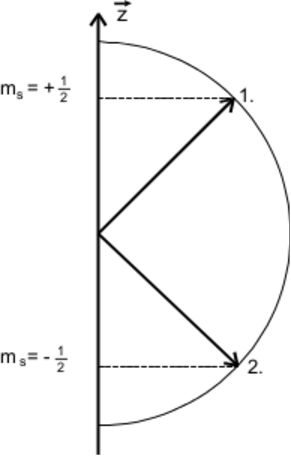
\includegraphics[width=\textwidth/4]{../Grafiken/SpinElektron.pdf}
\caption{Die Ausrichtung des Elektronen Spins bei einem Angeschaltetem Magnetfeld.\cite{V28}}\label{fig:Resonanz}
\end{figure}
\begin{align}
	\mu_{s_z}=-g\frac{1}{2}\mu_B
\end{align}
Dabei ist $g$ der Landé-Faktor oder auch gyromagnetisches  Moment genannt und wird eingeführt weil der Zusammenhang zwischen Spin und magnetischem Moment anders sein kann als beim Bahndrehimpuls.
Das, in diesem Versuch verwendete, homogene äußere Magnetfeld wurde durch ein Helmholtz-Spulenpaar erzeugt.
Die magnetische Feldstärke ergibt sich dabei aus dem Strom $I$ durch die Spule, der Windungszahl $N$ und
dem Spulenradius $R$ nach,
\begin{empheq}{equation}
	B(I) = \dfrac{8\cdot \mu_0}{\sqrt{125}} \cdot \dfrac{I\cdot N}{R}
	\label{eq:helmholtz}
\end{empheq}
  

\subsection{Elektronenspinresonanz}
\begin{figure}[h!]
\centering
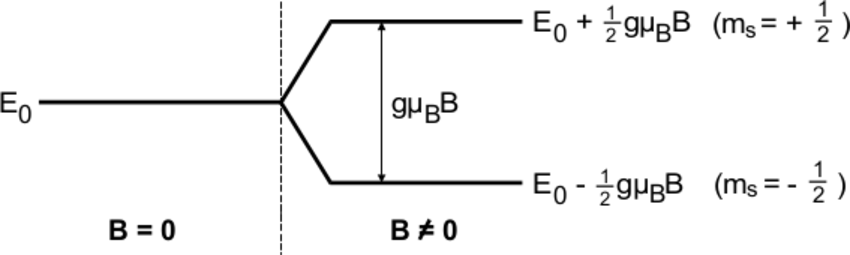
\includegraphics[width=\textwidth]{../Grafiken/EnergieAufspaltung.pdf}
\caption{Darstellung der Energie Aufspaltung.\cite{V28}}\label{fig:Resonanz}
\end{figure}
In diesem Versuch wird zur Bestimmung der gyromagnetischen Verhältnisses das Verfahren der Hochfrequenz Spektroskopie verwendet.\\
Es wird eine Substanz die freie Elektronen enthält, hier Diphenylpikrylhydrazyl, in ein homogenes Magnetfeld und teilt damit das Energieniveau in zwei auf. Die Differenz der beiden Niveaus ist dabei 
\begin{align}
	\Delta E = g\ \mu_B \ B.
\end{align}
Aus der Maxwell-Boltzmann-Statistik ist bekannt, dass das obere Energieniveau schwächer besetzt ist als das untere. Werden dem System jetzt Lichtquanten hinzugefügt, die die Energie 
\begin{align}
	\Delta E = g\ \mu_B \ B = h\nu=2\pi\hbar\nu
	\label{eq:energie}
\end{align}
wechseln die Elektronen das Energieniveau in das höhere und klappen ihren Spin um, dieser Prozess wird Elektronenspinresonanz genannt.
Die bei diesem Vorgang aufgenommene Energie geben die Elektronen durch Wechselwirkungsprozesse wieder ab. 

{ %TODO: Alte Version
%wechseln die Elektronen das Energieniveau in ein höheres und klappen ihren Spin um.

% Anmerkung: Das stimmt nicht, wir haben nur 10 - 30 MHz und es hat trotzdem funktioniert.
%Damit die Photonen diese Energie besitzen, müssen sie eine Frequenz $\nu$ in Größenordnung von 
%\SI{140}{\mega\hertz} besitzen.
% Anmerkung: Die Aufnahme der Energie und das Unklappen ist die SpinResonanz nicht die Abgabe der Energie.
%Die Elektronen geben ihre Energie durch Wechselwirkungsprozesse wieder ab. Dieser Prozess wird Elektronenspinresonanz genannt.	
}


